\maketitle


\tableofcontents
\newpage

\section{Bodenprognose (Meilensteine 5.1. und 5.2)}
Die Arbeiten im Berichtszeitraum fokussierten auf die  Entwicklung einer Prozesskette, die eine vergleichende Bewertung des Einflusses erklärender Variablen auf die Prognose von Bodenparametern und -klassen erlaubt. Die Prozesskette ist in Abbildung \ref{fig:scheme} dargestellt und läasst sich in die folgenden Schritte gliedern:

\begin{figure}[t]
    \centering
    \centering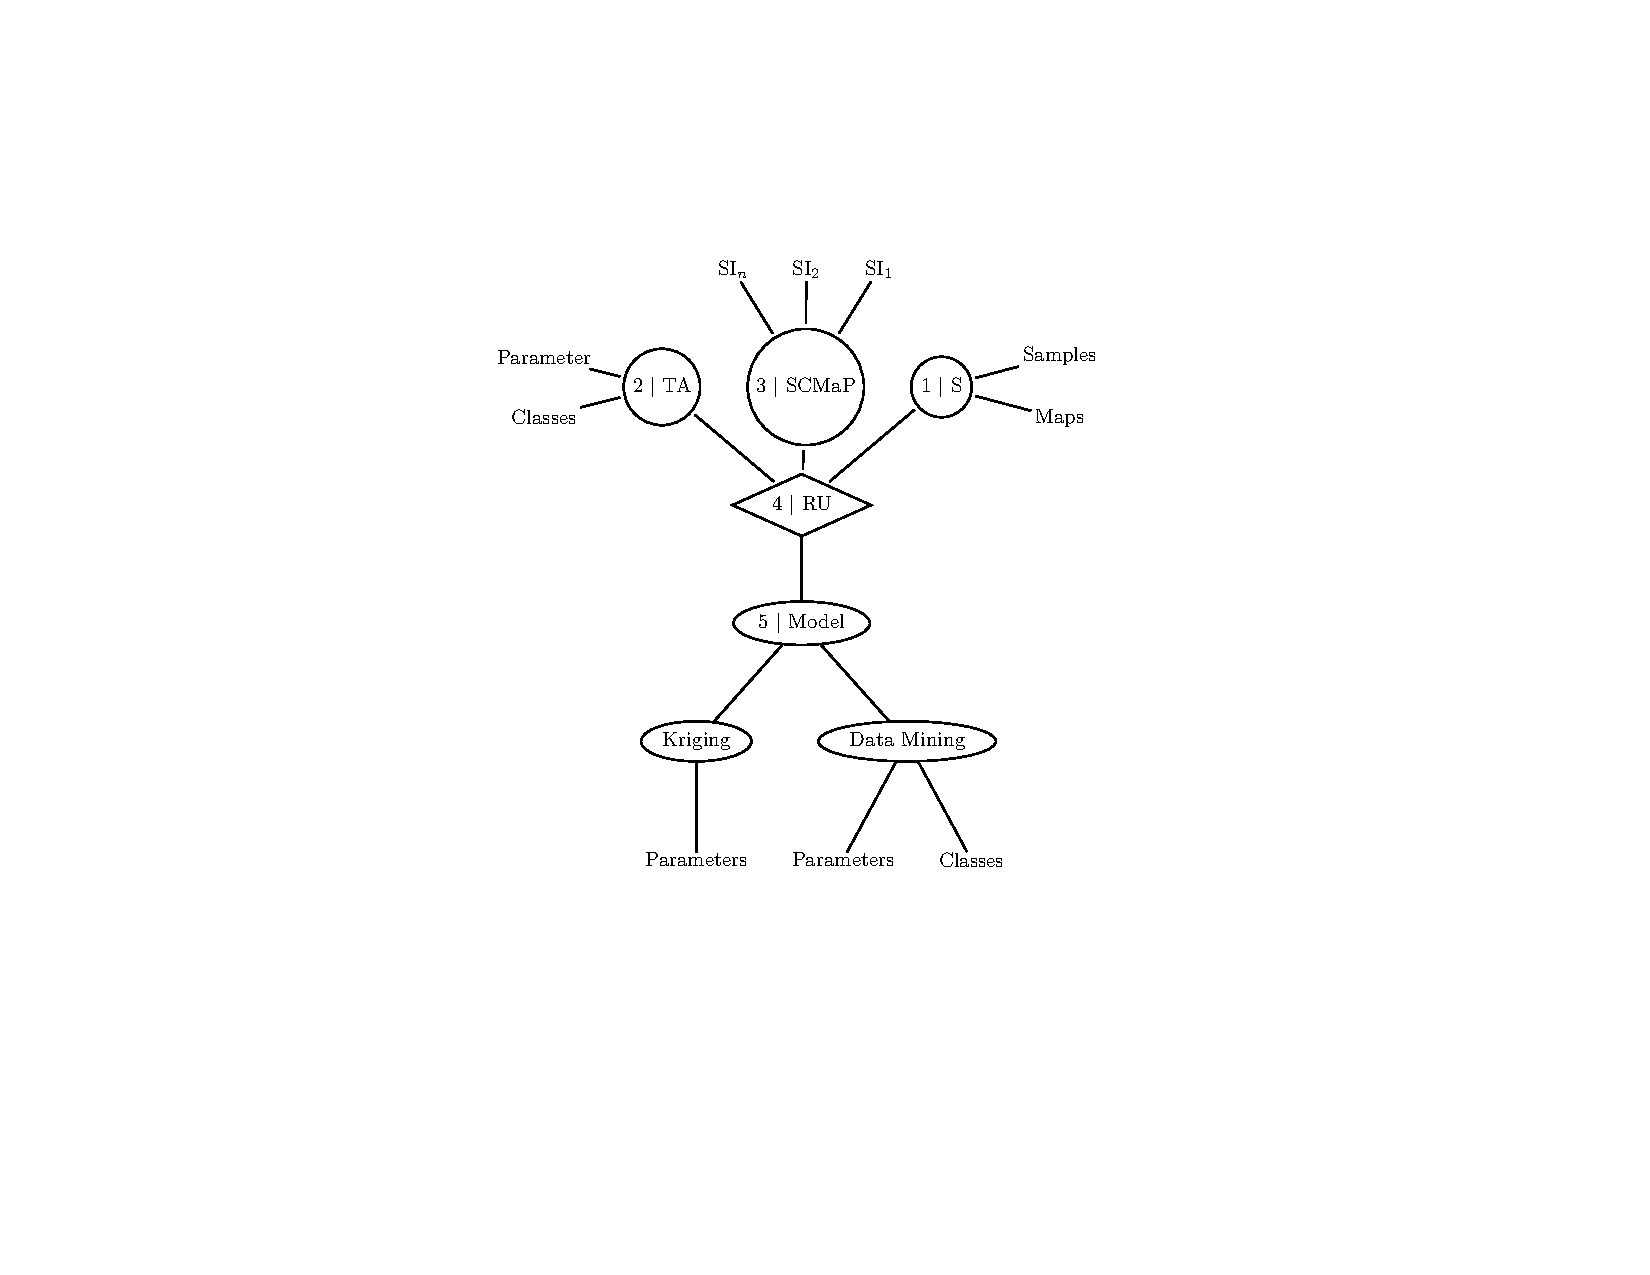
\includegraphics[width=0.6\textwidth]{figures/SOIL_DE_scheme.pdf}
    \caption{Fließschema zur maßstabsspezifischen Prognose von Bodeneigenschaften. SCMaP --  Soil Composite Mapping Processor $|$ S -- Bodendaten $|$ TA -- Reliefanalyse $|$ RU -- Bezugseinheit $|$ SR -- multi-temporale Spektralreflektanzen.}
    \label{fig:scheme}
\end{figure}

\begin{enumerate}
     \item Reliefinformationen (Parameter oder Klassen) ergeben sich aus der Anwendung von Reliefanalysealgorithmen (TA) auf digitale Höhenmodelle.
      \item Als bodenkundliche Datengrundlagen (S) dienen Aufschlüsse (Samples) oder Attribute bodenkundlicher Kartenwerke (Maps), die wiederum unterschiedliche Maß"-stäbe repräsentieren.
     \item Multi-temporale Reflektanzen (SR) sind das Ergebnis des Algorithmus \say{Soil Composite Mapping Processor} (Arbeitspaket AP\,4).
     \item Die Boden-, Relief- und Spektralinformationen werden mit Bezugseinheiten gekoppelt. 
     \item Bei der eigentlichen maßstabsspezifischen Prognose werden Verfahren des maschinellen Lernens angewendet.
 \end{enumerate}

Alle Schritte der Prozesskette innerhalb der Programmumgebung \textbf{R} in Form von Funktionen umgesetzt  \citep{R2018}. Die  Funktionen sind auf der Plattform GitHub\footnote{\url{https://github.com/terrasys/ScaleP}} abgelegt. 


\begin{table}[t]
	\centering
	\caption{Reliefattribute}\label{tab:terrainattributes}
	\begin{tabularx}{\textwidth}{l|X|X}
		\toprule
		\textbf{Abkürzung} & \textbf{Bedeutung} & \textbf{Quelle}\\
		\midrule
		$FILL$   & Digitales Höhenmodell  (= \textit{Digital Elevation Model}) mit gefüllten Senken &  \citep{PlanchonDarboux2001catena}\\\midrule
		$SLP$   & Hangneigung &  \citet{ZevenbergenThorne1987espl}\\\midrule
		$CA$   & Fließakkumulation &  \citet{Quinn-etal1991hp}\\\midrule
		$VDC$   & Vertical Distance above Channel network  &  \\\midrule
		$TCI$   & Terrain Classification Index (TCI) & \citet{Bock-etal2007saga}\\\midrule
		$TWI$   & Topographic Wetness Index &  \citet{BevenKirkby1979hsb}\\\midrule
		$MBI$   & Mass Balance Index &  \citet{Moeller-etal2008jpnss,Moeller-etal2012catena,MoellerVolk2015geoderma}\\\midrule
		$MRVBF$ & Multiresolution Index of Valley Bottom Flatness &  \citet{GallantDowling2003wrr}\\\midrule
		$TOP$   & Topographic (positive) Openness &  \citet{Yokoyama-etal2002pers}\\\midrule
	    $TON$   & Topographic (negative) Openness &  \citet{Yokoyama-etal2002pers}\\\midrule
		$NH$   & Relative Hangposition &  \citet{BoehnerSelige2006saga}\\\midrule
		$TPI$   & Topographic Position Index &  \citet{Guisan-etal1999pe}\\\bottomrule
	\end{tabularx}
\end{table}

\begin{table}[t]
	\caption{\texttt{fTerrA}: Parameter und Ergebnisdaten.}
	\centering
	\begin{tabularx}{\textwidth}{X|X}
		\toprule
		\textbf{Parameter/Ergebnisse} & \textbf{Bedeutung} \\
		\midrule
		\texttt{DEM.DIR} & Verzeichnis mit DEM\\ \midrule
		\texttt{DEM} & DEM-Name ohne Dateiformat \\ \midrule
	    \texttt{DEM.FRM} & DEM-Dateiformat\\ \midrule
		\texttt{OUT.DIR} & Ausgabeverzeichnis\\\midrule
		\texttt{EPSG} & DEM-Projektion entsprechend \url{https://spatialreference.org}\\\midrule
		\texttt{AGGREGATE} & Faktor zur Erhöhung der Rasterzellengröße\\\midrule
		\texttt{TA} & Präfix der resultierenden Reliefattributedateien\\\midrule
		\texttt{[TCI $|$ MBI $|$ NH $|$ TPI $|$ MRVBF] = TRUE} & Auswahl zu berechnender Reliefattribute\\\midrule
		\texttt{VECTOR = TRUE} & Vektorisierung des aggregierten \texttt{DEM}-Datensates\\
		\midrule
		\texttt{names\_TerrainAttributes.txt} & Bedeutung der Reliefattributdateien\\\midrule\midrule
		\texttt{[DEM]\_\text{AGGREGATE}[AGG]\_[TA][\dots].sgrd} & Namenskonvention der Reliefattributdateien (vgl. Tab. \ref{tab:terrainattributes})\\\midrule
		\texttt{[DEM]\_\text{AGGREGATE}[AGG]\_[TA].shp} & vektorisiertes aggregiertes Höhenmodell\\\midrule
		\texttt{[DEM]\_\text{AGGREGATE}[AGG]\_ [channel network][\dots].sgrd} & verschiedene Aggregierungsniveaus des Tiefenliniennetzes (channel network)\\\bottomrule
	\end{tabularx}
	\label{tab:fTerrA}%
\end{table}


\begin{table}[t]
	\caption{\texttt{fZonaSt}: Parameter und Ergebnisdaten.}
	\centering
	\begin{tabularx}{\textwidth}{l|X}
		\toprule
		\textbf{Parameter/Ergebnisse} & \textbf{Bedeutung} \\
		\midrule
		\texttt{TA.DIR} & Verzeichnis mit Reliefattributen [\texttt{*.sgrd}]\\ \midrule
		\texttt{TA} & Präfix der Reliefattribute und Spaltennamen der Ergebnisdatei\\\midrule
		\texttt{POLYGON.DIR} & Verzeichnis mit Polygonvektordatensatz (Bezugseinheiten)\\ \midrule
		\texttt{POLYGON.SHP} & Name des Polygonvektordatensatzes [\texttt{*.shp}]\\ \midrule
		%\texttt{ST} & Präfix der Fernerkundungsdaten und Spaltennamen der Ergebnisdatei\\\midrule
		\texttt{OUT.DIR} & Ausgabeverzeichnis\\\midrule\midrule
		\texttt{[DEM]\_\text{AGGREGATE}[AGG]\_[TA].shp} & Polygonvektordatensatz mit Reliefattributen
		\\\midrule
		\texttt{[DEM]\_\text{AGGREGATE}[AGG]\_[TA]\_CorMatr.csv} & Korrelationsmatrix aller Reliefattribute\\\bottomrule
	\end{tabularx}%
	\label{tab:fZonaSt}%
\end{table}


\subsection{Reliefanalyse}\label{sec:ta}
Zwischen Relief- und Bodeneigenschaften bestehen enge Beziehungen \citep{AGBoden2005}. Mit der flächen"-haften Verfügbarkeit von digitalen Reliefdaten sind Reliefableitungen und -klassi"-fi"-ka"-ti"-onen von besonderer Bedeutung für die digitale Prognose von Bodenklassen und -eigenschaften \citep{MinasnyMcBratney2016geoderma,Arrouays-etal2020geoderma}.\ 

Um der Maßstabsabhängigkeit von Bodeneigenschaften gerecht werden zu können, zielt die  Funktion \texttt{fTerrA()} zielt auf die Ableitung von bodenkundlich relevanten Reliefattributen, die verschiedene Aggregations- bzw. Maßstabsniveaus des Reliefs repräsentieren (Tab. \ref{tab:terrainattributes}). Das betrifft die Reliefattribute  $NH$ und $TPI$, für die Varianten mit verschiedenen \say{Moving Window}-Größen abgeleitet worden sind. Die Berechnungsvarianten der Reliefattribute $VDC$ und $TCI$ basieren auf verschiedenen Aggregationsniveaus des Tiefenliniennetzes. Die $MBI$-Versionen  sind schließlich Ausdruck von Varianten der Differenzierbarkeit von dominanten und subdominanten Reliefformen.\

\texttt{fTerrA()} ist in erster Linie eine Sammlung von Funktionen des \textbf{R}-Paketes \texttt{RSAGA} \citep{Brenning-etal2018}, worüber Funktionalitäten der Reliefanalysesoftware SAGA-GIS angesprochen werden können \citep{Conrad-etal2015gmd}. Tabelle \ref{tab:fTerrA} fasst die Parameter der Funktion \texttt{fTerrA()} zusammen, deren Aufruf dem Namen des digitalen Höhenmodells, dessen Dateiformat und Projektion sowie die Angabe eines Aggregierungsfaktor erfordert, mit dem wiederum die Rasterzzellengröße verändert werden kann. Zu"-sätz"-lich sind die Ergebnisdateien aufgelistet, die beim Aus"-führen der Funktion entstehen. Dazu gehören in erster Linie die Reliefattribute, die im SAGA GIS-Ras"-ter"-format \texttt{*.sgrd} vorgehalten werden. Die  darüber  hinaus abgeleiteten  \texttt{*.shp}-Dateien repräsentieren das vektorisierte aggregierte Höhenmodell (Polygonvektordatensatz) sowie verschiedene Aggregierungsniveaus des Tiefenliniennetzen (channel network; Linienvektordatensatz).




\begin{table}[p]
	\caption{\texttt{ClasP}: Parameter und Ergebnisdaten.}
	\centering
	\begin{tabularx}{\textwidth}{X|X}
		\toprule
		\textbf{Parameter/Ergebnisse} & \textbf{Bedeutung} \\
		\midrule
		\texttt{POLYGON.DIR} & Verzeichnis mit Polygonvektordatensatzes (Bezugseinheiten) \\ \midrule
		\texttt{POLYGON.SHP} & Vollständiger Name und Pfad des Polygonvektordatensatzes im \texttt{*.shp}-Format\\ \midrule
		\texttt{TRAIN.DIR} & Verzeichnis mit Trainingsdatensatz\\\midrule
		\texttt{TRAIN.SHP} & Trainingsdatensatz  im \texttt{*.shp}-Format\\\midrule
		\texttt{OUT.DIR} & Ausgabeverzeichnis \\\midrule
		\texttt{T.CLASS} & Spaltenname der Zielkategorie\\\midrule
		\texttt{M.TRAIN} & Methode des maschinellen Lernens (\url{https://topepo.github.io/caret/train-models-by-tag.html})\\\midrule
		\texttt{PART} & Verhältnis ($\in[0,1]$) zwischen Trainungs- und Testdatensatz\\\midrule
		\texttt{PF.TA} & \texttt{TRAIN.SHP}-Spaltennamen mit Reliefattributen\\\midrule
		\texttt{UP.TRAIN=TRUE} &  Ausgleich unbalanzieter Zielklassen im Trainingsdatensatz\\\midrule\midrule
		\texttt{[TRAIN.SHP]\_[T.CLASS]\_model- [M.TRAIN]\_part[PART].shp} & Trainingsdatensatz im \texttt{*.shp}-Format zur Modellbildung\\\midrule
		\texttt{[TRAIN.SHP]\_[T.CLASS]\_model- [M.TRAIN]\_part[PART].shp} & Testdatensatz im \texttt{*.shp}-Format zur Validierung\\\midrule
		\texttt{[TRAIN.SHP]\_[T.CLASS]\_model- [M.TRAIN]\_BP.shp} & Prozentuale Anteile der Zielklassen im Trainings- und Testdatensatz\\\midrule
		\texttt{[TRAIN.SHP]\_[T.CLASS]\_model- [M.TRAIN]\_VarImp.csv} & Bedeutung (Variable Importance) der erklärenden Variablen für die Prognose\\\midrule
		\texttt{[TRAIN.SHP]\_[POLYGON.SHP]\_[T.CLASS] \_MODEL-[M.TRAIN]\_part[PART].shp} & Prognoseergebnis mit den Spalten [T.CLASS\_SIM] und [T.CLASS\_PRB]\\\midrule
		\texttt{[TRAIN.SHP]\_[POLYGON.SHP]\_[T.CLASS] \_MODEL-[M.TRAIN]\_part[PART]\_CV.txt} & Gesamtgenauigkeit basierend auf Kreuzvalidierung\\\midrule
		\texttt{[TRAIN.SHP]\_[POLYGON.SHP]\_[T.CLASS] \_MODEL-[M.TRAIN]\_part[PART]\_CM.csv} & Konfusionsmatrix basierend auf der Prognose des Testdatesatzes\\\midrule
		\texttt{[TRAIN.SHP]\_[POLYGON.SHP]\_[T.CLASS] \_MODEL-[M.TRAIN]\_part[PART]\_AM.csv} & Genauigkeitsmaße basierend auf der Konfusionsmatrix\\\midrule
        \texttt{[TRAIN.SHP]\_[POLYGON.SHP]\_[T.CLASS] \_MODEL-[M.TRAIN]\_part[PART]\_BP.pdf} & Prozentuale Anteile der Zielklassen im Prognoseergebnis\\\bottomrule
		\end{tabularx}%
	\label{tab:fClasP}%
\end{table}




\subsection{Zonale Statistik}
Die Funktion \texttt{fZonaSt()} beinhaltet einen zonalen Statistikalgorithmus (Tab. \ref{tab:fZonaSt}), der Bestandteil der 
 \textbf{R}-Paketes \texttt{RSAGA} \citep{Brenning-etal2018} ist und die Verknüpfung von Rasterdaten und Bezugseinheiten erlaubt. Letztere repräsentieren bodenkundlich relevante Polygone, die beispielsweise aus der Verschneidung von verschiedenen Bodeneingangsdaten, aus der Segmentierung von Reliefattributen oder der Vektorisierung von Rasterzellen resultieren. Die Rasterdaten sind das Ergebnis der Funktionen \texttt{fTerrA()} (Kap. \ref{sec:ta}) und \texttt{fSCMaP()} (Kap. ???). 

\begin{table}[p]
	\caption{\texttt{NumP}: Parameter und Ergebnisdaten.}
	\centering
	\begin{tabularx}{\textwidth}{X|X}
		\toprule
		\textbf{Parameter/Ergebnisse} & \textbf{Bedeutung} \\
		\midrule
		\texttt{POLYGON.DIR} & Verzeichnis mit Polygonvektordatensatzes (Bezugseinheiten) \\ \midrule
		\texttt{POLYGON.SHP} & Vollständiger Name und Pfad des Polygonvektordatensatzes im \texttt{*.shp}-Format\\ \midrule
		\texttt{TRAIN.DIR} & Verzeichnis mit Trainingsdatensatz\\\midrule
		\texttt{TRAIN.SHP} & Trainingsdatensatz  im \texttt{*.shp}-Format\\\midrule
		\texttt{OUT.DIR} & Ausgabeverzeichnis \\\midrule
		\texttt{T.NUM} & Spaltenname des numerischen Zielparameters\\\midrule
		\texttt{M.TRAIN} & Methode des maschinellen Lernens (\url{https://topepo.github.io/caret/train-models-by-tag.html})\\\midrule
		\texttt{PART} & Verhältnis ($\in[0,1]$) zwischen Trainungs- und Testdatensatz\\\midrule
		\texttt{PF.TA} & \texttt{TRAIN.SHP}-Spaltennamen mit Reliefattributen\\\midrule\midrule
		\texttt{[TRAIN.SHP]\_[T.CLASS]\_model- [M.TRAIN]\_part[PART].shp} & Trainingsdatensatz im \texttt{*.shp}-Format zur Modellbildung\\\midrule
		\texttt{[TRAIN.SHP]\_[T.CLASS]\_model- [M.TRAIN]\_part[PART].shp} & Testdatensatz im \texttt{*.shp}-Format zur Validierung\\\midrule
		\texttt{[TRAIN.SHP]\_[T.CLASS]\_model- [M.TRAIN]\_DP.shp} & Dichtefunktionen (Density plot) des Trainings- und Testdatensatzes\\\midrule
		\texttt{[TRAIN.SHP]\_[T.CLASS]\_model- [M.TRAIN]\_VarImp.csv} & Bedeutung (Variable Importance) der erklärenden Variablen für die Prognose\\\midrule
		\texttt{[TRAIN.SHP]\_[POLYGON.SHP]\_[T.NUM] \_MODEL-[M.TRAIN]\_part[PART].shp} & Prognoseergebnis\\\midrule
		\texttt{[TRAIN.SHP]\_[POLYGON.SHP]\_[T.NUM] \_MODEL-[M.TRAIN]\_part[PART]\_CV.txt} & Gesamtgenauigkeit basierend auf Kreuzvalidierung\\\midrule
		\texttt{[TRAIN.SHP]\_[POLYGON.SHP]\_[T.NUM] \_MODEL-[M.TRAIN]\_part[PART] \_ACCtrain.csv} & Genauigkeitsmaße basierend auf der Prognose des Trainingsdatensatzes\\\bottomrule
		\texttt{[TRAIN.SHP]\_[POLYGON.SHP]\_[T.NUM] \_MODEL-[M.TRAIN]\_part[PART] \_ACCtest.csv} & Genauigkeitsmaße basierend auf der Prognose des Testdatensatzes\\\bottomrule
	\end{tabularx}%
	\label{tab:fNumP}%
\end{table}



\subsection{Modellierung}
Die Prognose der Zielklassen und numerischen Parameter basiert auf Algorithmen des maschinellen Lernens (= \textit{Data Mining}), die im \textbf{R}-Paket \texttt{caret} implementiert sind \citep{Kuhn2008jss,KuhnJohnson2013apm}. Die eigentliche Prognose wird mit dem im bodenkundlichen Kontext weit verbreitete und etablierte Entscheidungsbaumalgorithmus \say{Random Forest} durchgeführt \citep{Behrens-etal2018sr,Taghizadeh-Mehrjardi-etal2020}. Das Verfahren teilt unter optionaler Berücksichtigung von thematischen Klassen den n-dimensionalen Merkmalsraum von erklärenden Variablen solange, bis der höchste statistische Zusammenhang bei minimaler Varianz erreicht wird \citep{Breiman2001,LiawWiener2002}.\

Zur Validierung der Klassifikationsergebnisse wird der Gesamtdatensatz unter Berück"-sich"-ti"-gung der Zielklassen- bzw. Zielparameterverteilung in einen Trainings- und Testdatensatz von 75\,\% bzw. 25\,\% geteilt. Die Modellbildung basiert auf dem Trainingsdatensatz. Auf dessen Grundlage wird auch eine Kreuzvalidierung durchgeführt wird, aus der sich die Gesamtgenauigkeit des Modells ergibt. Der Testdatensatz dient der unabhängigen Validierung \citep{KhaledianMiller2020amm}, auf den das trainierte Modell angewendet wird. Zur Bewertung der numersichen Parameter dienen das Bestimmheitsmaß $R^2$ und das Streuungsmaß $RMSE$ (= \textit{Root Mean Square Error}). Die Beurteilung der prognostizierten Klassen wird mithilfe der klassenbezogenen F1-Werte und der Gesamtgenauigkeit vorgenommen. Der F1-Wert stellt das gewichtete harmonische Mittel aus Genauigkeit (\say{precision}) und Trefferquote (\say{recall}) einer jeden Klasse dar \citep{Manning-etal2008}: \say{precision} beschreibt das Verhältnis richtig klassifizierter Fälle zur Gesamtzahl der simulierten Fälle einer Klasse.  \say{recall} kennzeichnet das Verhältnis richtig klassifizierter Fälle zur Gesamtzahl der tatsächlichen Fälle einer Klasse. Die Gesamtgenauigkeit berechnet sich wiederum aus dem Verhältnis aller korrekten Treffer und der Gesamtzahl der Fälle berechnet \citep{Stehmann1997rse}.\

Die einzelnen Schritte der Klassifikationsprozedur sind in den Funktionen \texttt{fClasP()} und  \texttt{fNumP()} zusammengefasst. In den Tabellen  \ref{tab:fClasP} und \ref{tab:fNumP} sind die Parameter und Ergebnisdateien der Funktionen sowie deren Bedeutung aufgelistet. Neben dem Prognoseergebnis werden Dateien mit verschiedenen Genauigkeitsmaßen ausgegeben und visualisiert.

%\begin{enumerate}
%	\item Neben der Auswahl der Trainingsdaten (\texttt{TRAIN.SHP}) und parametrisierten Bezugseinheiten (\texttt{POLYGON.SHP}) kann durch den Nutzer die Option \texttt{UP.TRAIN} aktiviert werden, um der unbalanzierten Verteilung der Zielklassen zu begegnen \citep{Taghizadeh-Mehrjardi-etal2020}. Als Ergebnis werden das Prognoseergebnis mit den Spalten [T.CLASS\_SIM] (prognostizierte Klassen) und [T.CLASS\_PRB] (Wahrscheinlichkeit) ausgegeben. Letztere kennzeichnet der Anteil der Entscheidungsbaumanzahl, die zur klassenspezifischen Prognose geführt haben. Weiterhin werden verschiedene Dateien generiert, die die Prognosegüte basierend auf der Kreuzvalidierung sowie auf dem Testdatensatz beschreiben. Schließlich erlaubt der Vergleich der Klassenanteile im Testdatensatz und Prognoseergebnis eine Einschätzung der Plausibilität.
%	\item Bei der numerischen Prognose erfolgt nach Angabe des numerischen Zielparameters ebenfalls die Ableitung von Prognoseergebnissen und Genauigkeitsmaßen. 
%\end{enumerate}






\section{Bodenerosionsmodellierung (Meilenstein M5.3)}
$\dots$

\newpage
\bibliographystyle{apalike2}
\bibliography{references}









